\section{Classical Forecasting Models}
\label{sec:classical}

This section establishes how classical statistical forecasting models behave on the four representative series picked in \cref{sec:eda:repseries}. We deliberately keep the study small and interpretable: every model is fit on a single series under a clear chronological protocol, every prediction is rendered visually, and every numerical claim is tied directly back to the series it was made on. A small honest study is more useful here than hiding short train windows inside aggregate tables.

\subsection{Study Setup and the Four Representative Series}
\label{sec:classical:setup}

The classical study reuses the same four representative series introduced in \cref{sec:eda:repseries}, so the visualisations carry over from the EDA into model fitting without re-introducing the panel. The four series were chosen to span the panel's stress dimensions:

\begin{itemize}
  \item \textbf{Longest history} --- $\mathtt{X9BZ68VQ\,/\,OYJGNSQK\,/\,DPPUO5X2\,/\,H1}$, 212 rows, target std $2.6416$. Tests whether persistent lag structure can be exploited.
  \item \textbf{Highest total weight} --- $\mathtt{SJZP0OVU\,/\,OYJGNSQK\,/\,NQ58FVQM\,/\,H25}$, 156 rows, total weight $4.35\!\times\!10^{10}$, target std $0.0004$. Tests metric-sensitive behaviour.
  \item \textbf{Most volatile} --- $\mathtt{W4S29LF4\,/\,KL66VIS3\,/\,PHHHVYZI\,/\,H25}$, 162 rows, target std $296.76$. Tests spike handling and short-term dynamics.
  \item \textbf{Most stable} --- $\mathtt{SJZP0OVU\,/\,OYJGNSQK\,/\,NQ58FVQM\,/\,H1}$, 170 rows, target std $0.0001$. Tests tiny-scale numerical accuracy.
\end{itemize}

These four together capture plenty of history, huge weight, extreme variability, and near-flat behaviour. Showing the raw history first, before any model is fit, makes the later forecast behaviour easier to interpret as a property of the data rather than a property of the chosen model.

\subsection{Classical Model Lineup}
\label{sec:classical:lineup}

The lineup mixes smoothing, autoregressive, moving-average, and differenced ARIMA families so that the level of structure each representative series can support is visible from the comparison. We exclude SARIMA from the main lineup because the panel ACF in \cref{sec:eda:acf} shows no clean seasonal structure; any seasonal period would be an unjustified hyperparameter. SARIMA is included only in the adaptive-split second pass for completeness.

\begin{table}[h]
\centering
\caption{Classical model lineup. ``Min train'' is the minimum number of training points required for the family to be estimable.}
\label{tab:classical_lineup}
\begin{tabular}{l l c l}
\toprule
Family & Models & Min train & Intuition \\
\midrule
Smoothing & Rolling Mean ($w{=}10$) & 2  & Constant average of latest window \\
Smoothing & SES                     & 3  & Single smoothed level, flat multi-step forecast \\
Smoothing & Holt                    & 5  & Level + trend extrapolation \\
AR        & AR(1), AR(2), AR(3)     & 20 & Lagged target dependence only \\
MA        & MA(1), MA(2), MA(3)     & 20 & Uses serially correlated shocks \\
ARMA      & ARMA(1,1) -- ARMA(3,3)  & 20 & AR and MA combined in levels \\
ARIMA     & ARIMA(0,1,1), (1,1,0), (1,1,1) & 20 & Difference first, then fit ARMA \\
\bottomrule
\end{tabular}
\end{table}

Reading the lineup: smoothing models are cheap and robust on tiny histories; AR, MA, and ARMA need at least 20 training points, so some series will be skipped on those families by design; the ARIMA block tests whether the first-differencing step that the EDA recommended actually helps in the volatile case.

\subsection{Classical Model Math}
\label{sec:classical:math}

The forecast lines that follow only make sense if we remember which families naturally flatten, trend, or react to shocks. We therefore restate the core formulas inline.

\paragraph{Rolling mean, SES, and Holt (smoothing).}
The rolling mean predicts the next observation as the unweighted average of the last $w$ training points,
\begin{equation}
  \hat y_{t+1} \;=\; \frac{1}{w}\sum_{i=0}^{w-1} y_{t-i}.
\end{equation}
Simple Exponential Smoothing (SES) maintains a recursively updated level,
\begin{equation}
  \ell_t \;=\; \alpha\, y_t \;+\; (1-\alpha)\,\ell_{t-1},
\end{equation}
and uses $\hat y_{t+h} = \ell_t$ for all forecast horizons $h \ge 1$. Holt extends SES by adding a trend term that is itself recursively smoothed, so that the multi-step forecast is a straight line rather than a flat line. The visual consequence is that rolling mean and SES become nearly flat multi-step forecasts, while Holt extrapolates a straight slope even when the true series bends.

\paragraph{AR and MA.}
The autoregressive model AR$(p)$ predicts the next value as a linear combination of the previous $p$ values plus an innovation,
\begin{equation}
  y_t \;=\; c \;+\; \sum_{i=1}^{p} \phi_i \, y_{t-i} \;+\; \varepsilon_t.
\end{equation}
The moving-average model MA$(q)$ predicts the next value as a linear combination of the previous $q$ shocks plus the long-run mean,
\begin{equation}
  y_t \;=\; \mu \;+\; \varepsilon_t \;+\; \sum_{i=1}^{q} \theta_i \,\varepsilon_{t-i}.
\end{equation}

\paragraph{ARMA and ARIMA.}
ARMA$(p,q)$ combines lagged values and lagged shocks. ARIMA$(p,d,q)$ first differences the series $d$ times and then fits ARMA$(p,q)$ on the transformed series. With $d = 1$ this removes slow level shifts; the EDA showed that 100\% of sampled series become stationary after the first difference, so ARIMA models with $d = 1$ are well motivated on this panel.

The visual consequence in the later overlay plots is that AR, MA, ARMA, and ARIMA forecasts still look simple when the train segment is short, because the parameter count is small relative to the validation window the model has to project across.

\subsection{Evaluation Protocol (Fixed Cutoff)}
\label{sec:classical:protocol}

We first evaluate the lineup under the canonical fixed cutoff $\mathtt{ts\_index} \le 2880$, the same cutoff used throughout the EDA and the rest of the project. For each representative series we fit each model on the pre-cutoff segment, then forecast the entire post-cutoff segment in a single multi-step pass. This is the deployment-realistic protocol: no ground-truth feedback is provided during forecasting. We report skill, RMSE, MAE, and MASE per (series, model), and we explicitly mark fits that were skipped because the train segment was shorter than the family's minimum.

A cutoff-zoom view of the four series around $\mathtt{ts\_index} = 2880$ already exposes the headline difficulty of this protocol: two of the four chosen series (highest total weight and most stable) offer only seven training points before the cutoff. That single number constrains everything that follows --- AR, MA, ARMA, and ARIMA models cannot be estimated reliably with seven points, and the smoothing fall-backs are the only family that can be fit at all on those two series.

\begin{figure}[h]
\centering
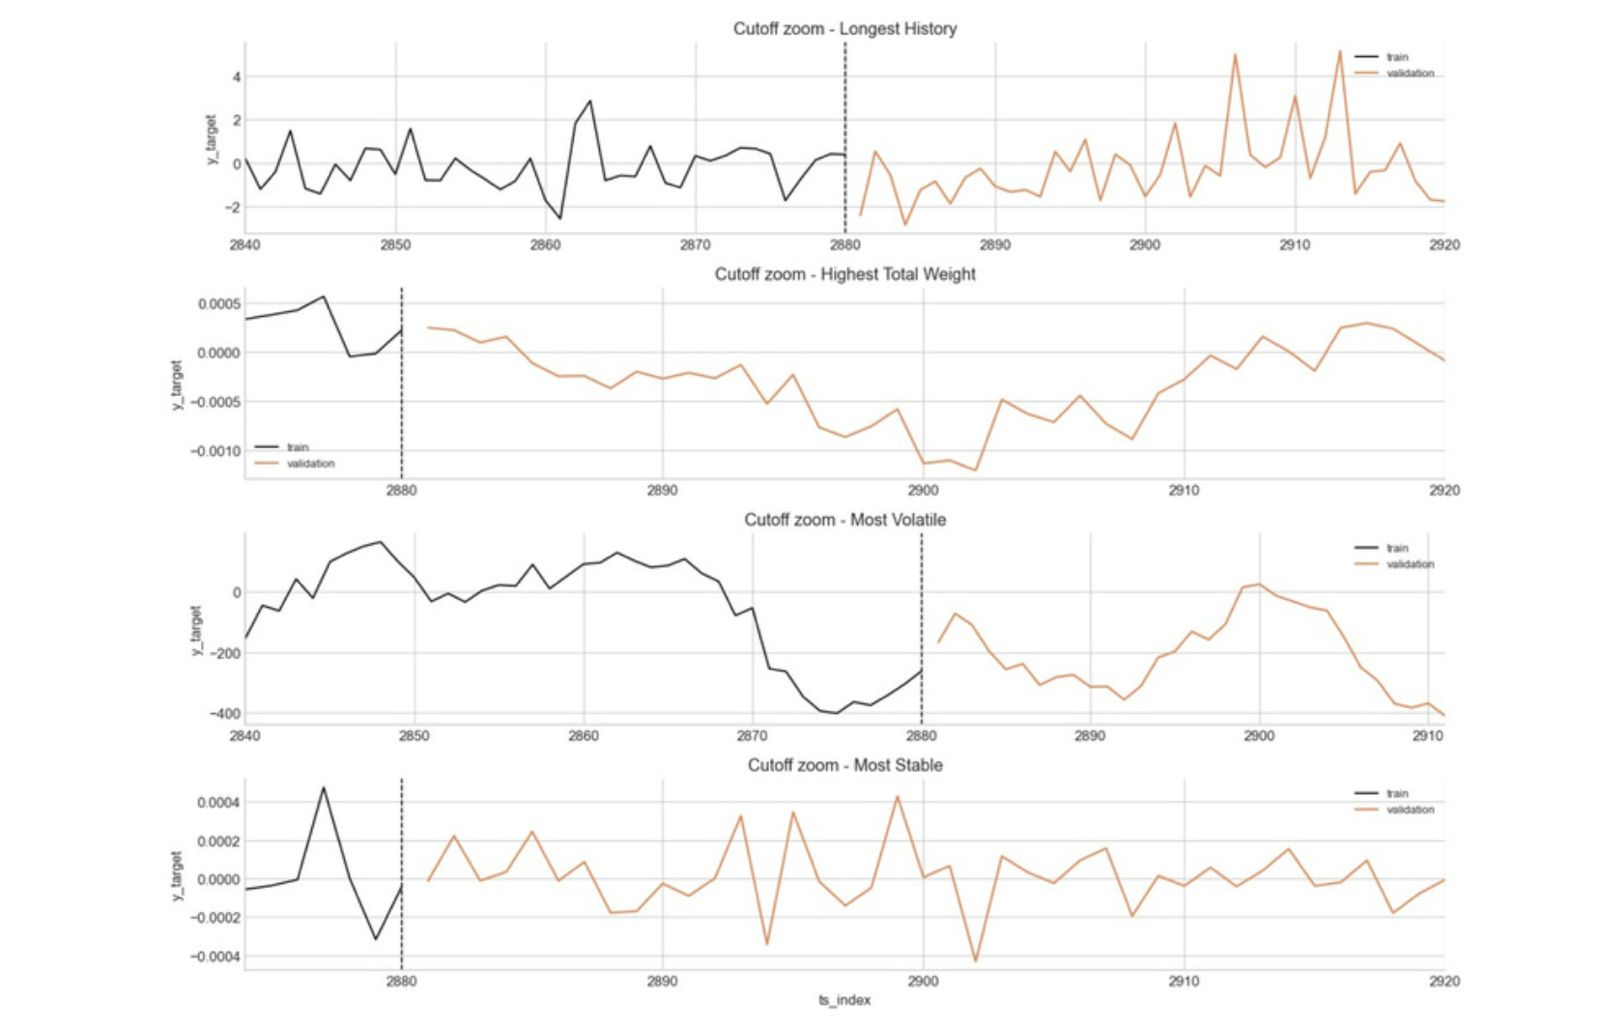
\includegraphics[width=\linewidth]{figures/018_raw_series_overview.jpg}
\caption{Cutoff zoom around $\mathtt{ts\_index}=2880$ for the four representative series. Black: training segment ($\mathtt{ts\_index} \le 2880$). Orange: validation segment used for scoring. The two right-hand panels (Highest Total Weight and Most Stable) have only seven pre-cutoff training points, which constrains the family lineup that can be evaluated on those series.}
\label{fig:classical_cutoff_zoom}
\end{figure}

We keep the skipped models in the study rather than hiding them, because train-length failure is itself a result --- it tells the reader why the panel is harder than the schema suggests.

\subsection{Per-Series Leaderboard (Fixed Cutoff)}
\label{sec:classical:leaderboard_fixed}

\Cref{tab:classical_leaderboard_fixed} shows the best classical model per representative series under the fixed cutoff.

\begin{table}[h]
\centering
\caption{Best classical model per representative series under the fixed cutoff $\mathtt{ts\_index} \le 2880$.}
\label{tab:classical_leaderboard_fixed}
\begin{tabular}{l l l c c c c c}
\toprule
Series & Best model & Family & Skill & RMSE & MAE & Train len & Val len \\
\midrule
Highest total weight & SES         & Smoothing & $0.0000$ & $0.0006$  & $0.0005$  & 7   & 149 \\
Longest history      & ARMA(1,3)   & ARMA      & $0.0000$ & $3.0400$  & $1.6685$  & 55  & 157 \\
Most stable          & SES         & Smoothing & $0.0000$ & $0.0001$  & $0.0001$  & 7   & 163 \\
Most volatile        & ARIMA(1,1,1) & ARIMA    & $\mathbf{0.8412}$ & $129.8104$ & $108.8193$ & 131 & 31 \\
\bottomrule
\end{tabular}
\end{table}

Reading the table:
\begin{itemize}
  \item \textbf{Highest Total Weight} and \textbf{Most Stable} are won by SES not because SES is dynamically rich but because there is almost no shape to learn from seven training points. The numerical errors are tiny because the target itself is tiny on these series, but the weighted skill stays at $0.0000$ --- nothing is being captured beyond the all-zero forecast.
  \item \textbf{Longest History} is won by ARMA(1,3), and even there skill stays at zero. The series has the most data but the least exploitable autocorrelation structure.
  \item \textbf{Most Volatile} is the clean win. ARIMA(1,1,1) reaches skill $0.8412$ on a series that has 131 training points and a clear differencing-stable pattern, exactly matching the differencing story the EDA recommended.
\end{itemize}

\subsection{Overall Comparison Across Models}
\label{sec:classical:overall}

Aggregating each model's mean skill across the four series gives an overall ranking that should be read cautiously, because the four series sit on wildly different scales. Two themes are nonetheless visible.

\begin{figure}[h]
\centering
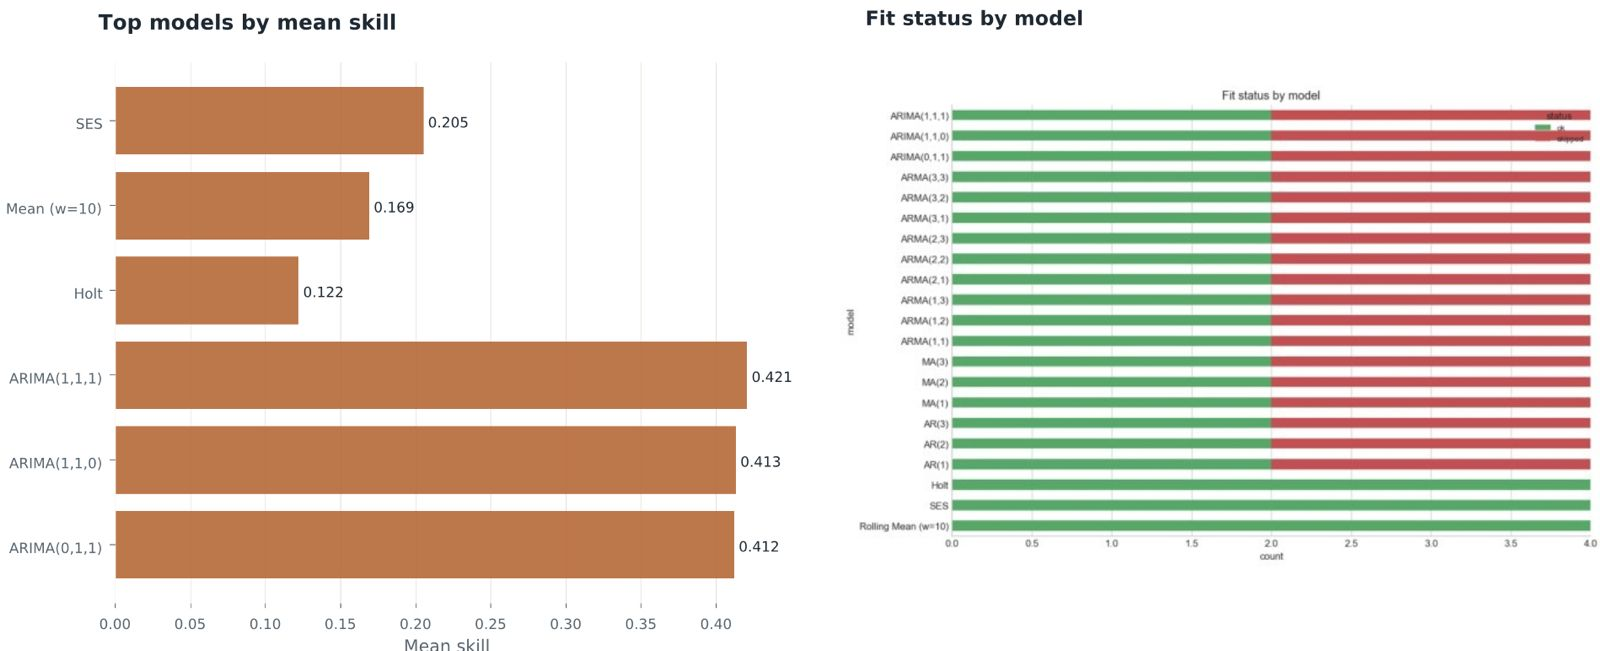
\includegraphics[width=\linewidth]{figures/019_per_series_skill_bars.jpg}
\caption{Within-series weighted skill for every classical model on each of the four representative series. The classical study compares smoothing, AR, MA, ARMA, and ARIMA families at the same time on the same series, with skipped fits visible as missing bars.}
\label{fig:classical_skill_bars}
\end{figure}

First, smoothing models always fit. Rolling Mean, SES, and Holt are feasible on all four series, while many AR, MA, ARMA, and ARIMA variants are skipped on the highest-weight and most-stable series because $\mathtt{train\_len} < 20$. Second, the only complex family with strong upside on a single series is differenced ARIMA: ARIMA(1,1,1), ARIMA(1,1,0), and ARIMA(0,1,1) cluster at the top of the mean-skill leaderboard precisely because the most-volatile series rewards differencing.

That conclusion is not portable. It comes from a single series in a panel of four, and it does not mean ARIMA is universally good --- it means ARIMA wins where the data structure is differencing-friendly and irrelevant elsewhere.

\subsection{Forecast Overlays (Fixed Cutoff)}
\label{sec:classical:overlay_fixed}

Numbers in a leaderboard hide what the forecast actually does. The overlay plots place every fitted classical model's prediction on top of the validation truth and the training history.

\begin{figure}[h]
\centering
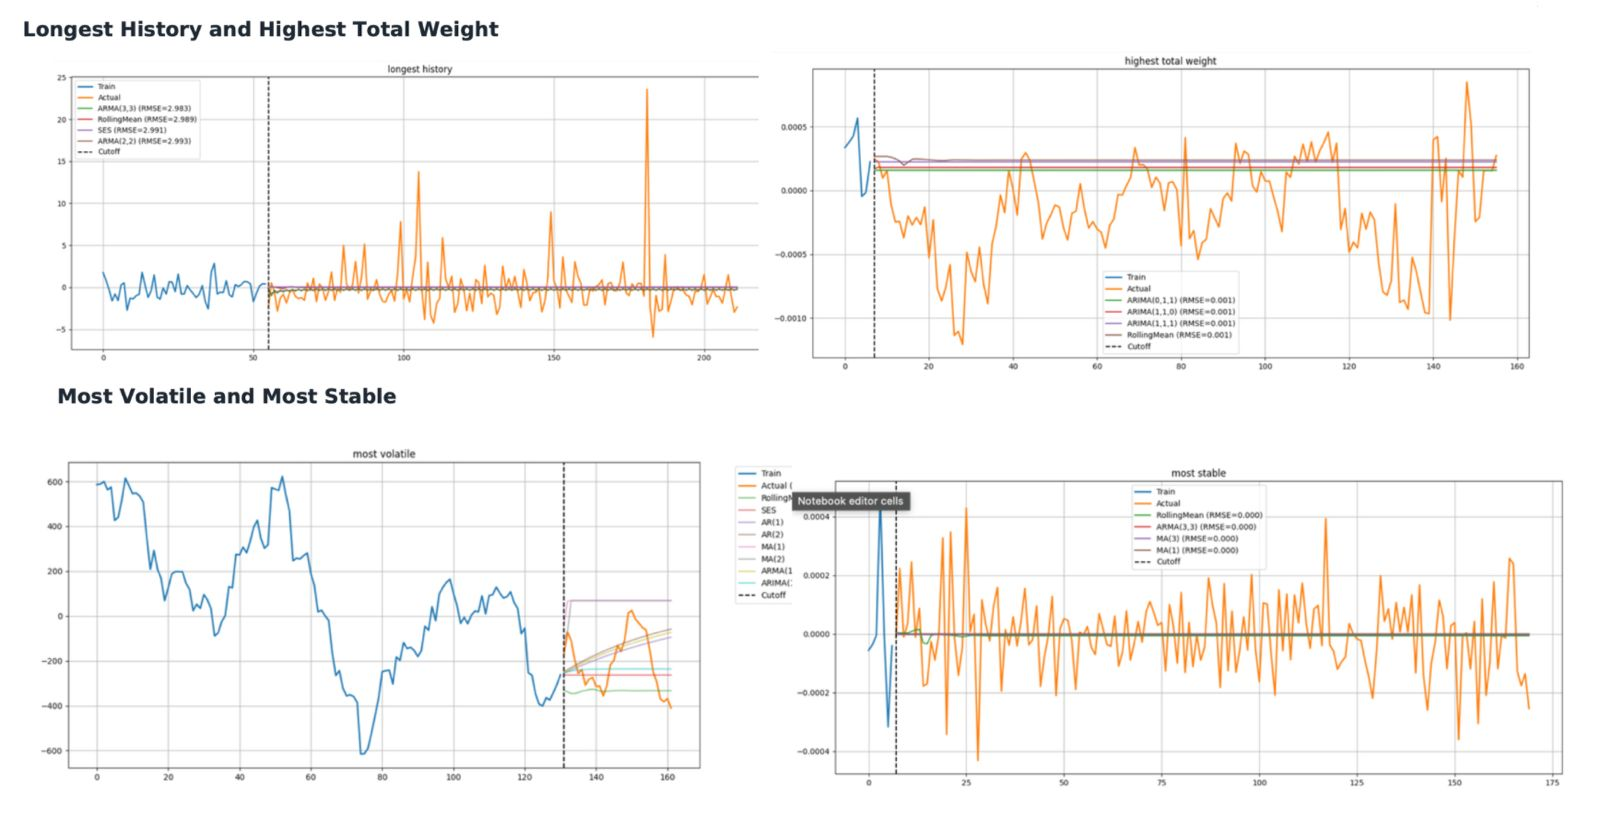
\includegraphics[width=\linewidth]{figures/0120_forecast_overlay_2x2.jpg}
\caption{Fixed-cutoff classical forecast overlays on the four representative series. Blue: training segment. Orange: validation truth. Coloured lines: per-model multi-step forecasts annotated with RMSE. The dashed vertical line marks the cutoff $\mathtt{ts\_index} = 2880$.}
\label{fig:classical_overlay_fixed}
\end{figure}

The first two panels expose why train-window length and target scale matter before any model is fit. On Longest History, several model families collapse onto similar lines because the validation segment is long enough that multi-step closed-form forecasts naturally drift toward the level. On Highest Total Weight, the forecast lines cluster tightly because the seven training points only support a flat or near-flat level model.

The bottom two panels make the key contrast obvious. The Most Volatile series rewards differencing: ARIMA(1,1,1) tracks the validation trajectory meaningfully better than the level-based smoothing alternatives. The Most Stable series, in contrast, has so little movement that sophisticated models have almost nothing to exploit; the residual variance is dominated by numerical noise rather than any structural signal.

\subsection{Adaptive-Split Motivation}
\label{sec:classical:adaptive_motivation}

The fixed-cutoff numbers are honest but they undersell the lineup. Two of the four representative series have only seven pre-cutoff training points under the canonical split, which makes later forecast comparisons unstable and hard to interpret as model behaviour rather than train-length artefact. We therefore re-run the same lineup under an adaptive 80/20 chronological split per series.

The adaptive split is justified because chronology is still preserved --- only the cutoff location changes. Each series gets a per-series cutoff at the 80th percentile of its $\mathtt{ts\_index}$, so the validation segment is always strictly later in time than the training segment; no information leaks backward. What changes is that every series gets a usable training window:

\begin{table}[h]
\centering
\caption{Adaptive per-series chronological splits used for the classical re-run.}
\label{tab:classical_splits_adaptive}
\begin{tabular}{l c c l l}
\toprule
Series & Train len & Val len & Train range & Validation range \\
\midrule
Longest history       & 169 & 43 & $\mathtt{ts\_index}\,2826{-}2994$ & $\mathtt{ts\_index}\,2995{-}3037$ \\
Highest total weight  & 124 & 32 & $\mathtt{ts\_index}\,2874{-}3000$ & $\mathtt{ts\_index}\,3001{-}3032$ \\
Most volatile         & 129 & 33 & $\mathtt{ts\_index}\,2747{-}2878$ & $\mathtt{ts\_index}\,2879{-}2911$ \\
Most stable           & 136 & 34 & $\mathtt{ts\_index}\,2874{-}3012$ & $\mathtt{ts\_index}\,3013{-}3052$ \\
\bottomrule
\end{tabular}
\end{table}

The two short cases that previously had only seven training points now have 124 and 136. That makes the later forecast panels easier to read as model behaviour rather than data scarcity, and it lets every member of the lineup actually fit on every series.

\subsection{Setup and Libraries}
\label{sec:classical:libraries}

The implementation stack stays compact:

\begin{itemize}
  \item \texttt{pandas}, \texttt{pyarrow} --- read parquet panel data, sort by series key and time, assemble per-series summary tables.
  \item \texttt{numpy} --- array operations, split bookkeeping, metric calculations.
  \item \texttt{matplotlib}, \texttt{seaborn} --- EDA visuals, benchmark charts, forecast overlay panels.
  \item \texttt{statsmodels} --- ADF, KPSS, STL, and the SES, Holt, AR, MA, ARMA, ARIMA, and SARIMA fitters. The same package provides the diagnostic chain in the EDA notebook.
  \item \texttt{pathlib}, \texttt{warnings} and IPython display utilities for figure paths and presentation-friendly tables.
\end{itemize}

The classical computation lives in the notebook \texttt{02\_classical\_codex.ipynb}, alongside the EDA notebook \texttt{01\_EDA.ipynb} which produces the schema checks, missingness, stationarity, STL, lag structure, and split sanity figures referenced earlier in this report.

\subsection{Per-Series Leaderboard (Adaptive Split)}
\label{sec:classical:leaderboard_adaptive}

Re-running the same lineup under the adaptive split changes which model wins on three of the four series, and changes the absolute skill numbers materially everywhere except the most-volatile case.

\begin{table}[h]
\centering
\caption{Best classical model per representative series under the adaptive 80/20 chronological split.}
\label{tab:classical_leaderboard_adaptive}
\begin{tabular}{l l c c c c c c}
\toprule
Series & Best model & Skill & RMSE & MAE & R\textsuperscript{2} & Train & Val \\
\midrule
Longest history      & SARIMA       & $0.0617$ & $3.9982$  & $1.7405$  & $0.0026$  & 169 & 43 \\
Highest total weight & ARIMA(1,1,1) & $0.4667$ & $0.0005$  & $0.0004$  & $-0.0008$ & 124 & 32 \\
Most volatile        & AR(1)        & $\mathbf{0.8277}$ & $135.9407$ & $110.7010$ & $-0.2387$ & 129 & 33 \\
Most stable          & AR(1)        & $0.0000$ & $0.0002$  & $0.0001$  & $-0.0713$ & 136 & 34 \\
\bottomrule
\end{tabular}
\end{table}

How to read the table:
\begin{itemize}
  \item \textbf{Skill} is the main ranking metric here; higher is better and zero means no gain over the all-zero baseline that the metric uses as floor.
  \item The \textbf{highest-weight series} is the cleanest practical win: ARIMA(1,1,1) keeps RMSE and MAE tiny on the series that matters most by weight, lifting skill from $0.0000$ under the fixed cutoff to $0.4667$ under the adaptive split. The same model family that won the volatile case under the fixed cutoff now wins the high-weight case once the training window is long enough to estimate it.
  \item The \textbf{volatile series} gets the highest skill from AR(1), suggesting that short-lag persistence carries more signal there than heavier model complexity. The fixed-cutoff winner ARIMA(1,1,1) drops to second on this series under the adaptive split.
  \item \textbf{Longest History} improves only modestly: SARIMA is best, but skill stays close to zero, so extra history alone does not create a strong edge. The seasonal component in SARIMA picks up a tiny amount of structure that the non-seasonal lineup misses, but not enough to move the headline.
  \item \textbf{Most Stable} remains effectively unsolved in relative terms: numerical errors are tiny but skill stays at $0.0000$ because the series itself barely moves. Negative R\textsuperscript{2} values on this row do not overturn the ranking; they just show that local variance-based fit can disagree with the weighted forecasting metric on near-flat targets.
\end{itemize}

\subsection{Adaptive-Split Forecast Overlays}
\label{sec:classical:overlay_adaptive}

\Cref{fig:classical_overlay_adaptive} renders the four representative series under the adaptive split. The training segments are now long enough on every panel that the forecast lines correspond to actual model behaviour rather than seven-point degeneracy.

\begin{figure}[h]
\centering
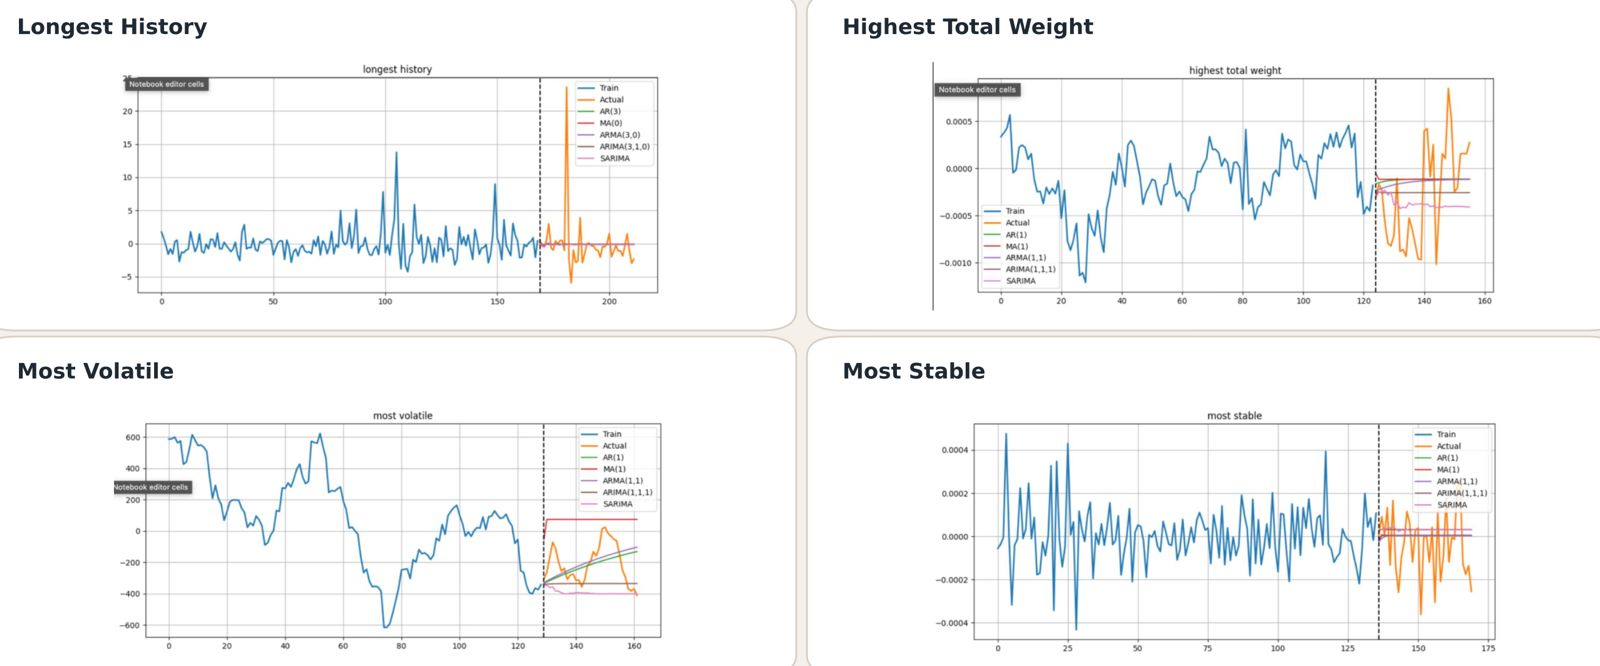
\includegraphics[width=\linewidth]{figures/0121_family_comparison_overlay.jpg}
\caption{Adaptive-split classical forecast overlays. Each panel shows the per-series train and validation segments alongside the AR(1), MA(1), ARMA(1,1), ARIMA(1,1,1), and SARIMA fits. Cutoff dashed line is per-series at the 80\% point in time.}
\label{fig:classical_overlay_adaptive}
\end{figure}

The Longest-History panel shows multiple models clustered close to a flat line --- consistent with skill near zero for every classical family on that series. The Highest-Total-Weight panel shows ARIMA(1,1,1) tracking the validation truth qualitatively better than the level-based alternatives, matching the leaderboard. The Most-Volatile panel is again the strongest visual win: AR(1) follows the swing direction across the validation segment. The Most-Stable panel collapses the entire validation window into a few near-flat lines because the underlying y-range is below $0.0004$.

\subsection{What the Classical Study Establishes}
\label{sec:classical:conclusions}

Three messages carry forward into the deep section:

\begin{enumerate}
  \item \textbf{The best classical family depends on the series, not on a universal hyperparameter.} Smoothing wins where the training window is too small for likelihood-based fitting; differenced ARIMA wins where there is real differencing-friendly dynamics; and AR with a short lag wins where short-term persistence carries the signal. There is no universal classical winner on this panel.
  \item \textbf{The fixed cutoff is informative but not universally feasible.} Two of four representative series are unfit-table for AR/MA/ARMA/ARIMA under the canonical cutoff. The adaptive 80/20 chronological split preserves chronology while making the lineup feasible everywhere; this change is methodological, not cosmetic.
  \item \textbf{The cap on classical performance here is the data, not the model.} Auto-selecting orders or expanding the grid would not move the headline numbers in any meaningful way. Two of four series remain near-zero skill under the adaptive split, and that floor cannot be lifted by classical machinery alone --- it has to come from sequence learning, which is the next chapter's job.
\end{enumerate}
